
\documentclass[10.9pt]{article}
%\usepackage[top=20mm,left=20mm,right=20mm,bottom=15mm,a4paper]{geometry} % see geometry.pdf on how to lay out the page. There's lots.
\usepackage[top=20mm,left=20mm,right=20mm,bottom=15mm,headsep=15pt,footskip=15pt,a4paper]{geometry} % see geometry.pdf on how to lay out the page. There's lots.
%\geometry{a4paper} % or letter or a5paper or ... etc
% \geometry{landscape} % rotated page geometry
\usepackage[round]{natbib}
\setlength{\bibsep}{0.0pt}
\usepackage{color}
\usepackage{times}
%\usepackage[T1]{fontenc}
%\usepackage{mathptmx}
\usepackage{tikz-dependency}
\usepackage{enumitem}
%\usepackage{times}

\usepackage[procnames]{listings}
\usepackage{color}
 
 

% See the ``Article customise'' template for come common customisations
\newcommand{\refeq}[1]{Equation~\ref{eq:#1}}
\newcommand{\reffig}[1]{Figure~\ref{fig:#1}}
\newcommand{\reftab}[1]{Table~\ref{tab:#1}}
\newcommand{\refsec}[1]{\textsection\ref{sec:#1}}
\newcommand{\newsec}[2]{\section{#1}\label{sec:#2}\noindent}
\newcommand{\newsubsec}[2]{\subsection{#1}\label{sec:#2}\noindent}
\newcommand{\argmax}{\operatornamewithlimits{argmax}} 
\newcommand{\argmin}{\operatornamewithlimits{argmin}} 

\makeatletter         
\def\@maketitle{   % custom maketitle 
\begin{center}%
{\bfseries \@title}%
{\bfseries \@author}%
\end{center}%
\smallskip \hrule \bigskip }

% custom section 
\renewcommand{\section}{\@startsection
{section}%                   % the name
{1}%                         % the level
{0mm}%                       % the indent
{-0.8\baselineskip}%            % the before skip
{0.3\baselineskip}%          % the after skip
{\bfseries\large}}% the style

% custom subsection 
\renewcommand{\subsection}{\@startsection
{subsection}%                   % the name
{2}%                         % the level
{0mm}%                       % the indent
{-0.8\baselineskip}%            % the before skip
{0.3\baselineskip}%          % the after skip
{\bfseries\large}}% the style

\renewcommand{\paragraph}{%
  \@startsection{paragraph}{4}%
  {\z@}{1.5ex \@plus 1ex \@minus .2ex}{-1em}%
  {\normalfont\normalsize\bfseries}%
}\makeatother

%\title{{\LARGE Universal Parser (UP)}\\[-8mm]
%\includegraphics[height=8mm]{RUPA}~~~~~~~~~~~~~~~~~~~~~~~~~~~~~~~~~~~~~~~~~~~~~~~~~~~~~~~~~~~~~~~~~~~~~~~~~~~\includegraphics[height=8mm]{RUPA}}
\title{{\LARGE Natural Language Processing}\\[1.5mm]{\large Lab 8: Dependency Annotation}}
\author{}
\date{} % delete this line to display the current date

%%% BEGIN DOCUMENT
\begin{document}

\definecolor{keywords}{RGB}{255,0,90}
\definecolor{comments}{RGB}{0,0,113}
\definecolor{red}{RGB}{160,0,0}
\definecolor{green}{RGB}{0,150,0}
 
\lstset{language=Python, 
        basicstyle=\ttfamily\small, 
        keywordstyle=\color{keywords},
        commentstyle=\color{comments},
        stringstyle=\color{red},
        showstringspaces=false,
        identifierstyle=\color{green},
        procnamekeys={def,class}}

\maketitle
%\tableofcontents
%\vspace{3mm}
\vspace{-2mm}
\newsec{Introduction}{intro}%
In this lab, we will perform grammatical annotation of English sentences, following the guidelines of the Universal Dependencies (UD) project.\footnote{{\tt http://universaldependencies.org}} The input to annotation will be text that has been tokenized, tagged and lemmatized, so the task will be limited to annotating syntactic structures
in the form of dependencies. 
We will use the UD Annotatrix tool for annotation and the MaltEval tool for comparing annotations. We will also need to consult the UD guidelines for syntactic annotation.\footnote{{\tt http://universaldependencies.org/u/overview/syntax.html}}

\newsec{Data}{data}%
The data to be annotated consists of 10 English sentences, selected from one of the English UD treebanks, stored in the file {\tt en10-anno.conll} 
(available in {\tt /local/kurs/nlp/syntax/}), and represented in the CoNLL-X format shown below.
\begin{center}
\fbox{
\lstinputlisting{code/tags.conll}
}
\end{center}
In this format, each word is represented by one line, consisting of tab-separated columns with the following interpretation:\footnote{For more information about the CoNLL-X format, see {\tt http://ilk.uvt.nl/conll/\#dataformat}. UD actually uses an evolved version of CoNLL-X called CoNLL-U, but the differences are irrelevant for this lab.} 
\begin{enumerate}[topsep=5pt,noitemsep]
\item ID: Word index, integer starting at 1 for each new sentence.
\item FORM: Word form or punctuation symbol.
\item LEMMA: Lemma or stem of word form.
\item CPOSTAG: Coarse-grained part-of-speech tag.
\item POSTAG: Fine-grained part-of-speech tag (same as CPOSTAG if not available).
\item FEATS: List of morphological features (underscore if not available).
\end{enumerate}
The syntactic dependency annotation will consist in adding two more columns:
\begin{enumerate}[topsep=5pt,noitemsep]
\item HEAD: Head of the current token, which is either a value of ID or zero (0).
\item DEPREL: Dependency relation to the HEAD (root iff HEAD = 0).
\end{enumerate}
However, instead of manipulating the CoNLL-X file directly, which would be theoretically possible but practically difficult and error-prone, we will use the Brat tool 
that provides a graphical user interface for annotation. 

\newsec{Start UD Annotatrix}{brat}%
UD Annotatrix is a web-based annotation tool available at: 
\begin{verbatim}
https://maryszmary.github.io/ud-annotatrix/standalone/annotator.html
\end{verbatim}
Load the file {\tt en10-anno.conll} by clicking on the ``import corpus" button and selecting the file. 
You should now see the first sentence in CoNLL-U format in the text window at the top of the screen. 
If you scroll down, you should also see a graphical display of the sentence, with words and tags but no dependencies, as shown below.
\begin{center}
\fbox{
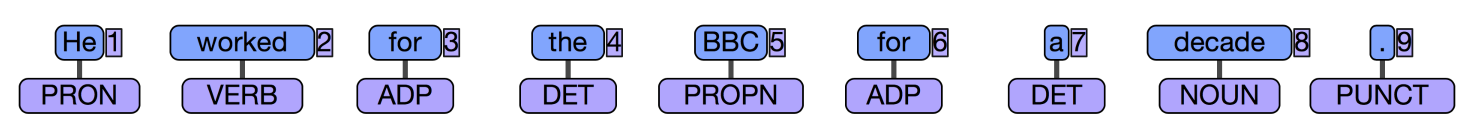
\includegraphics[scale=0.6]{pics/annotatrix}
}
\end{center}
You can now annotate dependency trees as follows:
\begin{enumerate}[topsep=5pt,noitemsep]
\item To add a dependency arc, click first on the head word and then on the dependent word.
\item To add a label to an arc, click on the arc and type the label (and hit the return key).
\item To remove a dependency arc, right-click to select and then hit the delete or backspace key.
\end{enumerate}
Note that the CoNLL-U representation at the top gets modified as well. In fact, you can also annotate by directly editing the CoNLL-U file. In general, we do not recommend doing this, because it is easier to make mistakes, but you have to use this method to add the root depependency. In other words, after you have added all dependencies between words, you should change the HEAD value to 0 and the DEPREL value to ``root'' for the word that is the root of the dependency tree. 

\paragraph{Important:} When you have finished the annotation, you must use the "Download corpus" button to download it to your computer. This puts it in the downloads folder, from which you may need to copy it to your working directory for the final comparison. 

\newsec{Annotate sentences}{annotate}%
When annotating a sentence, start by identifying the main predicate and annotate its core arguments.
\begin{center}
\fbox{
\begin{dependency}
\begin{deptext}[column sep=0.5cm]
This \& department \& now \& faces \& new \& challenges \& . \\[1mm]
DET \& NOUN \& ADV \& VERB \& ADJ \& NOUN \& PUNCT \\
\end{deptext}
%\depedge{2}{1}{det}
\depedge[edge style={red,thick}]{4}{2}{nsubj}
%\depedge{4}{3}{advmod}
%\depedge{6}{5}{amod}
\depedge[edge style={red,thick}]{4}{6}{obj}
%\depedge{4}{7}{punct}
\deproot[edge style={white}, edge unit distance=1.3em, hide label]{4}{}
\end{dependency}
}
\end{center}
Go on by annotating additional modifiers of the main predicate (including punctuation).
\begin{center}
\fbox{
\begin{dependency}
\begin{deptext}[column sep=0.5cm]
This \& department \& now \& faces \& new \& challenges \& . \\[1mm]
DET \& NOUN \& ADV \& VERB \& ADJ \& NOUN \& PUNCT \\
\end{deptext}
%\depedge{2}{1}{det}
\depedge{4}{2}{nsubj}
\depedge[edge style={red,thick}]{4}{3}{advmod}
%\depedge{6}{5}{amod}
\depedge{4}{6}{obj}
\depedge[edge style={red,thick}]{4}{7}{punct}
\deproot[edge style={white}, edge unit distance=1.3em, hide label]{4}{}
\end{dependency}
}
\end{center}
Then connect modifiers to the dependents of the main predicate (possibly in several steps).
\begin{center}
\fbox{
\begin{dependency}
\begin{deptext}[column sep=0.5cm]
This \& department \& now \& faces \& new \& challenges \& . \\[1mm]
DET \& NOUN \& ADV \& VERB \& ADJ \& NOUN \& PUNCT \\
\end{deptext}
%\depedge{2}{1}{det}
\depedge{4}{2}{nsubj}
\depedge{4}{3}{advmod}
\depedge[edge style={red,thick}]{6}{5}{amod}
\depedge{4}{6}{obj}
\depedge{4}{7}{punct}
\deproot[edge style={white}, edge unit distance=1.3em, hide label]{4}{}
\end{dependency}
}
\end{center}
Finally, attach function words to the content word they specify.
\begin{center}
\fbox{
\begin{dependency}
\begin{deptext}[column sep=0.5cm]
This \& department \& now \& faces \& new \& challenges \& . \\[1mm]
DET \& NOUN \& ADV \& VERB \& ADJ \& NOUN \& PUNCT \\
\end{deptext}
\depedge[edge style={red,thick}]{2}{1}{det}
\depedge{4}{2}{nsubj}
\depedge{4}{3}{advmod}
\depedge{6}{5}{amod}
\depedge{4}{6}{obj}
\depedge{4}{7}{punct}
\deproot[edge style={white}, edge unit distance=1.3em, hide label]{4}{}
\end{dependency}
}
\end{center}
Repeat the process for all 10 sentences, consulting the UD guidelines as needed.

\newsec{Compare annotations}{compare}%
When you have annotated all 10 sentences, you can either compare your annotations to those of another group or ask the lab instructor for the official UD annotation
(contained in the file {\tt en10-gold.conll}). What differences do you find? Did you make a mistake or do you want to argue for your analysis? Is it possible that more than
one analysis could be acceptable? You can visualize the differences using the MaltEval tool, which you can get by copying the file {\tt MaltEval.jar} from {\tt
  /local/kurs/nlp/syntax/}. If you want to compare two annotations that are stored in {\tt FILE1} and {\tt FILE2}, you can display both annotations with differences marked in red
  by running:
\begin{small}
\begin{verbatim}
java -jar -Xmx2g MaltEval.jar -g FILE1 -s FILE2 -v 1
\end{verbatim}
\end{small}
\end{document}
